\section{Весёлые интегралы в комплексной плоскости}

\begin{center}
\begin{longtable}{|p{0.03\textwidth}|p{0.3\textwidth}|p{0.6\textwidth}|}
	\hline
	\endfirsthead
	\hline
	\endhead
	\endfoot
	
	\hline
	\endlastfoot
	
	1 
	&
	
	$f(z)$ ограничена по модулю:
	\[
	|f(z)| < M
	\]
	
	\centering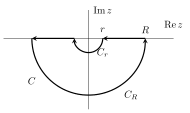
\includegraphics[width = 0.3 \textwidth]{images/png/countour_int1.png}
	&
	\[
	\begin{gathered}
	\oint\limits_C \frac{e^{-ia z}}{z} f(z) dz = 
	\int\limits_{C_R} + \int\limits_{R}^{r} + \int\limits_{C_r} + \int\limits_{-r}^{-R}
	\end{gathered}
	\]
	\[
	\begin{gathered}
	\left|
	\int\limits_{C_R} \frac{e^{-ia z}}{z} f(z) dz 
	\right| 
	= \left| 
	\int\limits_{\pi}^{2\pi} i e^{-ia R e^{i\varphi}} f(R e^{i\varphi}) d\varphi
	\right|
	\leqslant 
	\int\limits_{\pi}^{2\pi} e^{a R \sin \varphi} M d \varphi = \\ =
	M e^{a R \sin \varphi^*} \pi\Big|_{\varphi^* \in (\pi, 2\pi)} \underset{R \to \infty}{\to} 0
	\end{gathered}
	\]
	\[
	\begin{gathered}
	\lim\limits_{r \to 0} \int\limits_{C_r} \frac{e^{-ia z}}{z} f(z) dz =
	\lim\limits_{r \to 0} \int\limits_{2\pi}^{\pi} i e^{-ia R e^{i\varphi}} f(r e^{i\varphi}) d\varphi =
	- i f(0) \pi
	\end{gathered}
	\]
	\[
	\begin{gathered}
	\fint\limits_{-\infty}^{\infty} \frac{e^{-ia z}}{z} f(z) dz =
	- i f(0) \pi
	\end{gathered}
	\]
	Можно показать, что при изменении знака $a$ изменится контур (будет вверху), направление обхода и как следствие знак результата.
	\[
	\begin{gathered}
	\fint\limits_{-\infty}^{\infty} \frac{e^{ia z}}{z} f(z) dz =
	i f(0) \pi \sign a
	\end{gathered}
	\]
	Отсюда можно получить более общее выражение:
	\[
	\begin{gathered}
	\fint\limits_{-\infty}^{\infty} \frac{e^{ia z}}{z - z_0} f(z) dz =
	i e^{iaz_0} f(z_0) \pi \sign a
	\end{gathered}
	\]
	\\ 
\end{longtable}
\end{center}